\section{Electromagnetism}
(such as electrostatics, currents and DC
circuits, magnetic fields in free space,
Lorentz force, induction, Maxwell’s
equations and their applications,
electromagnetic waves, AC circuits,
magnetic and electric fields in matter)

\subsection{Electrostatics}
\Table{
\hline

$\epsilon$ is called... 	& permittivity %\\
%and has units ...		& Farads per meter (F/m) = 

\\ \hline

$\mu$ is called & permeability

\\ \hline

Gauss's Law & Flux $\Phi \equiv \oint \bold{E} \cdot d\bold{a} = Q_{enc} / \epsilon_0 \Leftrightarrow $ M.E. I

\\ \hline
}

%%%%

\Table{
\hline

E-field for sphere of radius R with 	& $E_{inside} = \dfrac{Q}{4 \pi \epsilon_0} \dfrac{r}{R^3}$ \\
uniformly distributed charge Q		& $E_{outside} = \dfrac{Q}{4 \pi \epsilon_0} \dfrac{1}{r^2}$

\\ \hline

Electric Potential	& $ V(\bold{a}) = - \int_0^a \bold{E}(\bold{r}) \cdot d\bold{l} $\\
				& $ V(a) - V(b) = \int_a^b \bold{E}(\bold{r}) \cdot d \bold{l} $
				
\\ \hline

Energy of a point charge & $W=QV$

\\ \hline
}

%%%%

\Table{
\hline

Energy of a collection of point charges 	& $ U = \dfrac{1}{8 \pi \epsilon_0} \sum_{j=0}^n \sum_{i=0, i\neq j}^{n} \dfrac{q_i q_j}{r_{if}} $ \\
								& $ U = \dfrac{1}{2} \sum_{all \ i} V_{due \ to \ others} (r_i)q_i $.

\\ \hline

\MiniPg{.4}{

\center

Energy of a continuous distribution of charge

}

&


\MiniPg{.6}{
\center

$W = \dfrac{1}{2} \int_V \rho V d \tau = \dfrac{\epsilon_0}{2} \int_{all space} E^2 d\tau $.

}

\\ \hline

Energy density of $E$ field

&

$\eta_E = \dfrac{1}{2}\epsilon E^2$	

\\ \hline
}

%%%%

\Table{
\hline

\MiniPg{.3}{
Conductor:  $\bold{E}_{inside} $, $\rho_{inside} $, $V(r) = $, $\hat{E}_{surface} $
}

&

\MiniPg{.7}{

 $\bold{E}_{inside} = \bold{0} \ \ \ \ \ \ \rho_{inside} = 0 \ \ \ \ \ \ V(r) = constant \ \ \ \ \ \ \hat{E}_{surface}  = \bot_{surface}$
}

\\ \hline
}

%%%%

\Table{
\hline
			& $\bold{E} (\bold{r}) = \dfrac{1}{4\pi \epsilon_0} \iiint_{volume} \dfrac{1}{R^2} \rho (\bold{r}') d\tau' \hat R$ \\
Coulomb's Law	& $\bold{E} (\bold{r}) = \dfrac{1}{4\pi \epsilon_0} \iint_{surface} \dfrac{1}{R^2} \sigma (\bold{r}') da' \hat R$ \\
			&  $\bold{E} (\bold{r}) = \dfrac{1}{4\pi \epsilon_0} \int_{line} \dfrac{1}{R^2} \lambda (\bold{r}') dl' \hat R$

\\ \hline

Coulomb Potential	&  $V (\bold{r}) = \dfrac{1}{4\pi \epsilon_0} \int \dfrac{1}{R} \rho (\bold{r}') d\tau' $

\\ \hline

}

%%%%

\Table{
\hline

Poisson's Equation	& $\nabla^2V = -\rho / \epsilon_0$ \\
Laplace's Equation	& $\nabla^2V = 0 $ 

\\ \hline

}


%%%%

\Table{
\hline


\begin{minipage}{.3\textwidth}
      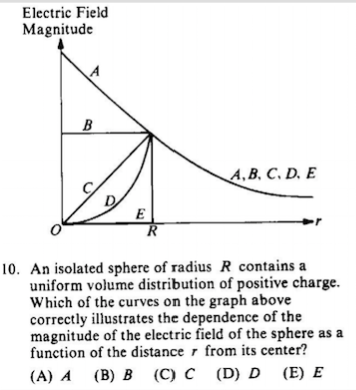
\includegraphics[width=\linewidth, height=60mm]{images/ChargeSphereUniform.png}
      \tiny \url{GR8677}
    \end{minipage}

& C

\\ \hline

Given $R$ and either $Q$ or $\rho$ find & $E(r<R) = \dfrac{Qr}{4 \pi \epsilon_0 R^3} = \dfrac{\rho r}{3 \epsilon_0} $ \\


E-field inside sphere and & \\


 outside sphere & $E(r>R) = \dfrac{Q}{4 \pi \epsilon_0 r^2} = \dfrac{\rho R^3}{3 \epsilon_0 r^2} $

\\ \hline

}

%%%%%

\Table{
\hline

Griffith's triangle of $\rho, V \& \bold{E}$ &

\begin{minipage}{.4\textwidth}
      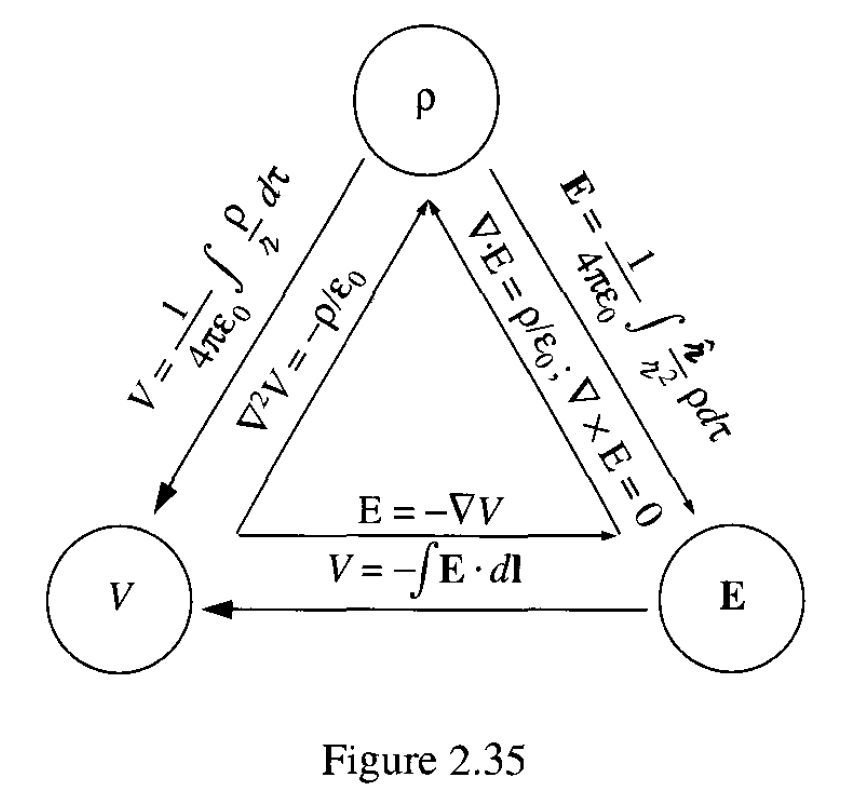
\includegraphics[width=\linewidth, height=60mm]{images/GriffithsTriangle.png}
      \tiny \textit{Introduction to Electrodynamics}, Griffiths
    \end{minipage}
    
\\ \hline
}

%%%%

\Table{
\hline

\MiniPg{.3}{

Electric potential for multipole expansion (far field)

}

&

\MiniPg{.7}{

\GraphicWHN{.76}{.2}{Mulitpole.png}
\center

\small Fig. 3.27 in Griffiths, \textit{Introduction to Electrodynamics}

}

\\ \hline
}

%%%%

\Table{
\hline

\MiniPg{.3}{

Electric dipole moment

}

&

\MiniPg{.7}{
\center

$\bold{p} \equiv \int \bold{r}' \rho{\bold{r}'} \, d\tau'$

For point charges, $\bold{p} = \sum_{i = 1}^{n} q_i \bold{r}_i'$.

}

\\ \hline
}

%%%%

\Table{
\hline

\MiniPg{.3}{

Electric potential for dipole

}

&

\MiniPg{.7}{
\center

$V_{\textrm{dip}}(\bold{r}) = \dfrac{1}{4 \pi \epsilon_0 } \dfrac{ \bold{p} \cdot \bold{\hat{r}} }{r^2} = \dfrac{p \ \cos \theta}{4 \pi \epsilon_0 r^2}$.

}

\\ \hline
}

%%%%

\Table{
\hline

\MiniPg{.3}{

Electric field of a dipole

}

&

\MiniPg{.7}{
\center

$\bold{E}_{\textrm{dip}}(\bold{r}) = \dfrac{1}{4 \pi \epsilon_0} \dfrac{1}{r^3} [3(\bold{p} \cdot \bold{\hat{r}})\bold{\hat{r}} - \bold{p}]$.

$\bold{E}_{\textrm{dip}} (r, \theta) = \dfrac{p}{4 \pi \epsilon_0 r^3} (2 \cos \theta  \,\bold{\hat{r}} + \sin \theta \,\pmb{\hat{\theta}})$.

\GraphicWHN{.4}{.32}{Dipole.png}

\center
\small Fig. 3.36 from Griffiths, \textit{Introduction to Electrodynamics}

}

\\ \hline
}

%%%%%%%%%%%%%%%%%%%%%%%%%%%%%%%%%%%%%

\subsection{Capacitors}
\Table{
\hline

Capacitance & $C = \dfrac{q}{V}$

\\ \hline

Voltage/current relationship & $I(t) = C\dfrac{dV(t)}{dt}$

\\ \hline

Charging energy & $W_{\textrm{charging}} = \dfrac{1}{2} C V^2$

\\ \hline
}

%%%%

\Table{
\hline

Capacitance of a capacitor

& 

\MiniPg{.6}{

Mutual capacitance between two conducting plates, i.e. a regular capacitor, is given by

$C = \epsilon_r \epsilon_0 \dfrac{A}{d}$.

}

\\ \hline
}

%%%%%%%%%%%%%%%%%%%%%%%%%%%%%%%%%%%%%%%

\subsection{Currents and DC}
\Table{
\hline

Amperes = & Coulombs / second
 
 \\ \hline

Ohm's Law & $V=IR$

\\ \hline
}

%%%%

\Table{
\hline
 
Current in a wire of area $A$, & \\
velocity of charges $v$, & $I = v \rho A$ \\
 charge density $\rho$ &

\\ \hline
}

%%%%

\Table{
\hline

\MiniPg{.3}{Kirchoff's current law}

&

\MiniPg{.7}{

The algebraic sum of currents in a network of conductors meeting at a point is zero.

}

\\ \hline

\MiniPg{.3}{Kirchoff's voltage law}

&

\MiniPg{.7}{

The directed sum of the electrical potential differences (voltage) around any closed network is zero.

}

\\ \hline
}

%%%%

\Table{
\hline

RC circuit $V(t)$ where $V(0)=V_0$

&

\MiniPg{.6}{
\center

Start with Kirchoff's current law for a circuit consisting of just a capacitor and a resistor.

 $C\dfrac{dV}{dt} + \dfrac{V}{R} = 0$
 
Solve the DE.

$\boxed{ V(t) = V_0e^{-\frac{t}{RC}}}$

}

\\ \hline
}

%%%%

\Table{
\hline

RL circuit voltages across R and L

&

\MiniPg{.6}{ \center
 $V_L(t) = V e^{-t \frac{R}{L}} $
  
$V_R(t) =V(1 - e^{-t \frac{R}{L}})$
}
\\ \hline
}



%%%%%%%%%%%%%%%%%%%%%%%%%%%%%%%%%%%%%%%%



\subsection{Magnetic fields in free space}

\Table{
\hline

Biot-Savart Law & $\bold{B} = \dfrac{\mu_0}{4\pi} \int \dfrac{\bold{I} \times \hat R}{R^2} dl' = \dfrac{\mu_0 I}{4\pi} \int \dfrac{\bold{dl'} \times \hat R}{R^2} $

\\ \hline

Ampere's law	& $\oint \bold{B} \cdot d\bold{l} = \mu_0 I_{enc} $

\\ \hline
}

%%%%

\Table{
\hline

\MiniPg{.3}{

B-field for solenoid with $n$ turns per unit length and current $I$.

}

&

$\bold{B} = \mu_0 n I \hat z $

\\ \hline
}

%%%

\Table{
\hline

B-field for infinite wire

&

$B = \dfrac{\mu_0 I}{2 \pi r}$

\\ \hline
}

%%%%

\Table{
\hline

\begin{minipage}{.3\textwidth}

Field on axis of current loop.

General, $z=0$, and $z>>R$


\end{minipage}

& 

\MiniPg{.7}{
\GraphicWHN{.7}{.54}{MagCurLoop.png}

\center

\tiny \url{http://hyperphysics.phy-astr.gsu.edu/hbase/magnetic/curloo.html}

\large

$B = B_Z = \dfrac{\mu_0}{4 \pi} \dfrac{2 \pi R^2 I}{(z^2 +R^2)^{3/2}} =\boxed{\dfrac{\mu_0}{2} \dfrac{R^2 I}{(z^2 +R^2)^{3/2}}}$

If $z = 0$ then $\boxed{B = \dfrac{\mu_0 I}{2R} }$.

If $z>>R$ then $\boxed{B \approx \dfrac{\mu_0}{2} \dfrac{R^2 I}{z^3}}$

}

\\ \hline
}

%%%%

\Table{
\hline

Magnetic vector potential	& $\bold{B} = \bold{\nabla} \times \bold{A} 	$\\
					&$ \bold{A} \parallel  \bold{J} $ \\
					&$ \bold{A}(\bold{r}) = \dfrac{\mu_0}{4 \pi} \int \dfrac{\bold{J}(\bold{r}')}{R} d\tau' $ \\
					&$ \oint \bold{A} \cdot d \bold{l} = \Phi_B $

\\ \hline

}

%%%%

\Table{
\hline

\MiniPg{.3}{

Griffiths triangle for magnetostatics 

}

&

\MiniPg{.7}{

\GraphicWHN{.5}{.5}{MagTriangle.png}

\center
\small Griffiths, \textit{Introduction to Electrodynamics}

}

\\ \hline
}

%%%%

\Table{
\hline

\MiniPg{.3}{

Magnetic vector potential for magnetic dipole

}

&

\MiniPg{.7}{
\center

$ \bold{A}_{\textrm{dip}} (\bold{r}) = \dfrac{\mu_0}{4 \pi} \dfrac{\bold{m} \times \bold{\hat{r}}} {r^2} $

$\bold{A}_{\textrm{dip}} (\bold{r}) = \dfrac{\mu_0}{4 \pi} \dfrac{m \, \sin \theta}{r^2} \pmb{\hat{\phi}}$.

}

\\ \hline

Magnetic dipole moment

&

$\bold{m} \equiv I \int d\bold{a} = I \bold{a}$

\\ \hline
}

%%%%

\Table{
\hline

\MiniPg{.3}{

Magnetic field of magnetic dipole

}

&

\MiniPg{.7}{
\center

$\bold{B}_{\textrm{dip}}(\bold{r}) = \dfrac{\mu_0}{4 \pi} \dfrac{1}{r^3} [3( \bold{m} \cdot \bold{\hat{r}}) \bold{\hat{r}} - \bold{m}].$


$\bold{B}_{\textrm{dip}} (\bold{r}) = \dfrac{ \mu_0 m}{4 \pi r^3} (2 \cos \theta \bold{\hat{r}} + \sin \theta \pmb{\hat{ \theta}})$.

\GraphicWHN{.35}{.3}{MagDipole.png}

\center

\small Fig. 5.54 from Griffiths, \textit{Introduction to Electrodynamics}

}

\\ \hline
}

%%%%

\Table{
\hline

Potential energy associated with magnetic moment

& 

$U(\theta) = - \pmb{\mu} \cdot \bold{B}$

\\ \hline
}

%%%%

\Table{
\hline

Larmor precession

&

\MiniPg{.7}{
\center
$\pmb{\tau} = \pmb{\mu} \times \bold{B}$. This causes centripetal acceleration (think of the poles of the magnet).

\MPalign{

\dfrac{dL}{dt} &= \tau \\
 \dfrac{L \sin \theta d\phi}{dt} &= |\mu B \sin \theta| \\
 \omega_{\textrm{precession}} &= \dfrac{\mu B}{L}
 
}
}

\\ \hline
}

%%%%%%%%%%%%%%%%%%%%%%%%%%%

\subsection{Lorentz force}

\Table{
\hline

The Lorentz Force & $ \bold{F} = q(\bold{E} + \bold{v} \times \bold{B})$

\\ \hline
}

%%%%

\Table{
\hline
\MiniPg{.3}
{
Magnetic force on a current carrying wire of length $l$ and current $I$ in a field $\bold{B}$
}
&
\MiniPg{.6}
{

\center

$\bold{F} = q \bold{v} \times \bold{B} = qvB (\hat{v} \times \hat{B}) = q\dfrac{l}{t}B (\hat{v} \times \hat{B})  = \dfrac{q}{t} l B (\hat{v} \times \hat{B}) = \boxed{ I l B (\hat{v} \times \hat{B}) }$

%\begin{tabular}{c c}
%$\bold{F}$&$= q \bold{v} \times \bold{B}$ \\
%	 &$= qvB (\hat{v} \times \hat{B})$ \\
%	 &$= q\dfrac{l}{t}B (\hat{v} \times \hat{B}) $\\
%	 &$= \dfrac{q}{t} l B (\hat{v} \times \hat{B})$ \\
%	 &$= \boxed{ I l B (\hat{v} \times \hat{B}) }$
% \end{tabular}

}
 
 \\ \hline
}

%%%%

\Table{
\hline

\MiniPg{.25}{
Larmor radius, cyclotron or gyroradius rather
}

&

\MiniPg{.75}{
\center

A charged particle traveling perpendicular to a magnetic field will gyrate in a circle whose area vector is parallel to the direction of travel resulting in a corkscrew-like trajectory. The radius of gyration is determined by considering the Lorentz force on such a particle.

$\dfrac{mv_{\bot}^2}{r_g} = |q|v_{\bot}B \Rightarrow \boxed{r_g = \dfrac{mv_{\bot}}{|q|B}}$

}

\\ \hline
}

%%%%

\Table{
\hline

Cyclotron frequency

&

\MiniPg{.7}{

\MPalign{
T_g &= \dfrac{2 \pi r_g}{v_{\bot}} = \dfrac{2 \pi}{v_{\bot}} \dfrac{mv_{\bot}}{|q|B} = \dfrac{2 \pi m}{|q|B} \\
f_g &= \dfrac{|q|B}{2 \pi m} \\
\omega_g &= \dfrac{|q|B}{m}
}

}


\\ \hline
}



%%%%%%%%%%%%%%%%%%%%%%%%%%%%%%%


\subsection{Induction}
\Table{
\hline

Faraday's/Lenz's law

&

\MiniPg{.6}{
\center
If an induced current flows, its direction is always such that it will oppose the change which produced it.

$\varepsilon = -\dfrac{d \Phi_B}{dt}$

}

\\ \hline
}

%%%%

\Table{
\hline

\MiniPg{.4}{

EMF for tightly wound coil of wire

}

&

$\varepsilon = -N\dfrac{d \Phi_B}{dt}$

 \\ \hline

Inductance & $L \equiv \dfrac{\Phi_B}{I}$

\\ \hline
}

%%%%

\Table{
\hline

Voltage, given inductance & $V = \dfrac{d}{dt}(LI) = L \dfrac{dI}{dt}$

\\ \hline

Energy in an inductor

&

$W = \int P \ dt = \int IV \ dt = \int I L \dfrac{dI}{dt} dt = L \int I \ dI = \boxed{\dfrac{1}{2} L I^2}.$

\\ \hline
}

%%%%

\Table{
\hline

\MiniPg{.3}{
Energy density in magnetic field
}
&

\MiniPg{.7}{
\center

$\eta_B =  \dfrac{W}{V}  = \dfrac{ \frac{1}{2} LI^2  }{A l} = \dfrac{1}{2} \dfrac{\frac{\Phi_B}{I} I^2}{A l} = \dfrac{1}{2} \dfrac{BAI}{Al}  = \dfrac{1}{2} \dfrac{BI}{l} .$


But in a solenoid, we have $\bold{B} = \mu n I \hat{z} = \dfrac{\mu I}{l}$, so $\dfrac{I}{l} = \dfrac{B}{\mu}$. Therefore, $\boxed{\eta_B = \dfrac{1}{2} \dfrac{B^2}{\mu}}$.

}

\\ \hline
}

%%%%%%%%%%%%%%%%%%%%%%%


\subsection{Maxwell's Equations}

\Table{
\hline

Maxwell's equations 	& $\pmb{\nabla} \cdot \bold{E} = \rho / \epsilon_0 $ (Gauss) \\
in vacuum. 		& $\pmb{\nabla} \cdot \bold{B} = 0 $ \\
Differential form	& $\pmb{\nabla} \times \bold{E} = -\dfrac{\partial \bold{B}}{\partial t} $ (Faraday) \\
				& $\pmb{\nabla} \times \bold{B} = \mu_0\bold{J} + \epsilon_0 \mu_0 \dfrac{\partial \bold{E}}{\partial t} $ (Ampere)

\\ \hline
}

%%%%
\Table{
\hline

Maxwell's equations 	& $\oiint\limits_{\partial \Omega} \bold{E} \cdot d\bold{S} = \dfrac{1}{\epsilon_0} \iiint_\Omega \rho dV$ (Gauss) \\
in vacuum. 		& $\oiint_{\partial \Omega} \bold{B} \cdot d\bold{S} = 0$ \\
Integral form		& $\oint_{\partial \Sigma} \bold{E} \cdot d\bold{l} = -\dfrac{d}{dt} \iint_\Sigma \bold{B} \cdot d\bold{S}$ (Faraday) \\
				& $ \oint_{\partial \Sigma} \bold{B} \cdot d \bold{l} = \mu_0 \iint_\Sigma \bold{J} \cdot d\bold{S} + \mu_0\epsilon_0 \dfrac{d}{dt} \iint_\Sigma \bold{E} \cdot d\bold{S} $ (Ampere)

\\ \hline
}

%%%%
\Table{
\hline

\MiniPg{.3}{
\center

Maxwell's equations in matter.
Differential form
}
&
\MiniPg{.7}{
\center
$\pmb{\nabla} \cdot \bold{D} = \rho_{free}  $ (Gauss), \, \, \, 
\small $D = \epsilon_0 E + P, \, \, \, \, \, D = \epsilon E$

\large

$\pmb{\nabla} \cdot \bold{B} = 0 $ \\

$\pmb{\nabla} \times \bold{E} = -\dfrac{\partial \bold{B}}{\partial t} $ (Faraday) \\

$\pmb{\nabla} \times \bold{H} = \bold{J}_{free} + \dfrac{\partial \bold{D}}{\partial t} $ (Ampere), \, \, \,
\small $B = \mu_0(H + M), \, \, \, \, \, B = \mu H$
\large

}
\\ \hline
}


\Table{
\hline

Maxwell's equations 	& $\oiint\limits_{\partial \Omega} \bold{D} \cdot d\bold{S} = \iiint_\Omega \rho_{free} dV$ (Gauss) \\
in matter. 		& $\oiint_{\partial \Omega} \bold{B} \cdot d\bold{S} = 0$ \\
Integral form		& $\oint_{\partial \Sigma} \bold{E} \cdot d\bold{l} = -\dfrac{d}{dt} \iint_\Sigma \bold{B} \cdot d\bold{S}$ (Faraday) \\
				& $ \oint_{\partial \Sigma} \bold{H} \cdot d \bold{l} = \iint_\Sigma \bold{J}_{free} \cdot d\bold{S} + \dfrac{d}{dt} \iint_\Sigma \bold{D} \cdot d\bold{S} $ (Ampere)

\\ \hline
}

\Table{
\hline
Boundary conditions

&
\MiniPg{.7}{

\MPalign{

(i)&  D^\bot_1 - D^\bot_2 = \sigma_f \\

(ii)& B^\bot_1 -B^\bot_2 = 0 \\

(iii)&  \bold{E^{||}_1} - \bold{E^{||}_2} = 0 \\

(iv)&  \bold{H^{||}_1} - \bold{H^{||}_2} = \bold{K}_f \times \bold{ \hat{n}}
}

}

 \\ \hline
}

%======================================================%

\subsection{EM Waves}
\Table{
\hline
\MiniPg{.2}{ The whole EM wave spiel}

&

\MiniPg{.8}{
		\center
		For E-wave, curl Faraday.
		
		$\nabla \times \nabla \times \bold{E} = \nabla \times \Big(-\dfrac{\partial B}{\partial t} \Big)$ 

		$\nabla (\nabla \cdot \bold{E} ) - \nabla^2 \bold{E}  = -\dfrac{\partial}{\partial t} (\nabla \times \bold{B}) $
		
		Substitute Gaussian and Amperian terms.
		
		$\nabla \Big(\dfrac{\rho}{\epsilon_0}\Big) - \nabla^2 \bold{E}  = -\dfrac{\partial}{\partial t} \Big(\mu_0\bold{J} + \epsilon_0 \mu_0 \dfrac{\partial \bold{E}}{\partial t}\Big) $
		
		$\rho = 0$ and $\bold{J} = 0$, therefore  $\boxed{\nabla^2 \bold{E} = \epsilon_0 \mu_0 \dfrac{\partial^2 \bold{E} }{ \partial t^2} = \dfrac{1}{c^2}\dfrac{\partial^2 \bold{E} }{ \partial t^2} }$
		
		For B-wave, similar, but start with curling Ampere's Law.
	}
	
\\ \hline
}

%%%%

\Table{
\hline

speed of light in vacuum & $c = \dfrac{1}{\sqrt{\mu_0 \epsilon_0}} = 3 \times 10^8$ m/s 

\\ \hline

speed of light in medium, $v= $& $\dfrac{1}{\sqrt{\mu \epsilon}} = \dfrac{c}{\sqrt{\epsilon_R \mu_R}}$, where $\mu = \mu_R \mu_0$ and likewise for $\epsilon$

 \\ \hline

 Plane wave solutions & $E = E_m \sin(kx - \omega t)$ and $ B = B_m\sin(kx - \omega t)$
 
 \\ \hline
}

%%%%

\Table{
\hline
 
 \MiniPg{.3}{
 Relation of $E_m$ and $B_m$ magnitudes
 }
 
 &
 
 \MiniPg{.7}{ Plug plane wave solutions into Ampere or Faraday and find that
 \center
 $\dfrac{E_m}{B_m} = \dfrac{\omega}{k} = c$
 
 }
 
 \\ \hline
}

%%%%

\Table{
\hline

\MiniPg{.3}{

Energy in the E and B fields for plane wave

}

&

\MiniPg{.7}{
\center


Recall the energy densities $\eta_E = \dfrac{1}{2} \epsilon_0 E^2$ and $\eta_B = \dfrac{1}{2} \dfrac{B^2}{\mu_0}$.

$\dfrac{\eta_E}{\eta_B} = \dfrac{\mu_0 \epsilon_0 E^2}{B^2} = \dfrac{E^2}{c^2 B^2}$.

From above, $E = cB$. Therefore $\eta_E = \eta_B$ for an EM wave; the energy carried in the E-field is equal to the energy carried in the B-field.

}

\\ \hline
}

%%%%

\Table{
\hline

Poynting Vector

& 

\MiniPg{.6}{
\center
	
$\bold{S} = \dfrac{1}{\mu_0} \bold{E} \times \bold{B}$

$S = \dfrac{1}{\mu_0} EB = \dfrac{c}{\mu_0} B^2 = \dfrac{1}{c\mu_0} E^2 $

}

\\ \hline
}

%%%%

\Table{
\hline

Average intensity

&

$\overline{S} = \dfrac{1}{c \mu_0} E^2_m \overline{\sin^2(kx - \omega t)} = \dfrac{1}{c \mu_0} \dfrac{E_m^2}{2}$
	
\\ \hline

\MiniPg{.4}{

Power radiated by a non relativistic point charge as it accelerates

}

&

\MiniPg{.6}{
\center

Larmor formula

$P = \dfrac{2}{3}\dfrac{q^2 a^2}{4 \pi \epsilon_0 c^3} = \dfrac{q^2 a^2}{6 \pi \epsilon_0 c^3} $.

}


	
\\ \hline
}


%%%%%

\Table{
\hline

\MiniPg{.4}{
Application of boundary conditions for reflection of a wave incident to a conducting surface
}

&

\MiniPg{.6}{

(i) Incident wave, $E^\bot = 0$ on both sides $\rightarrow \, \sigma_f = 0$ 

(ii) Automatically satisfied because $B^\bot = 0$

(iii) $\tilde{E}_{0_I} + \tilde{E}_{0_R} = \tilde{E}_{0_T}$

(iv)

\GraphicWHN{1}{.6}{ivEMWaveCond.png}

Wave is reflected with $\pi$ phase shift. Also, from the last equation above, $\tilde{B}_{0_R} = -\tilde{B}_{0_I}, \ \ \tilde{B}_{0_T} = 0$. From the first expression it follows that the magnetic field at the surface is twice the magnitude of either incident or reflected. 

\tiny \textit{Introduction to Electrodynamics}, Griffiths

}

\\ \hline

}

%%%%

\Table{
\hline

Oscillating electric dipole

&

\MiniPg{.6}{
\center

$q(t) = q_0 \cos(\omega t) \;\;\;\;\;\;\; \bold{p}(t) = p_0 \cos(\omega t) \bold{\hat{z}} \;\;\;\;\;\;\; p_0 \equiv q_0 d.$

}

\\ \hline
}

%%%%

\Table{
\hline

\MiniPg{.4}{

Approximations for oscillating electric dipole far from the source (such that it can be approximated as a plane wave)

}

&

\MiniPg{.6}{
\center

Approximation 1: $d \ll r$.

Approximation 2: $d \ll \dfrac{c}{\omega} = \dfrac{\lambda}{2 \pi}$.

Approximation 3: $r  \gg  \dfrac{c}{\omega} = \dfrac{\lambda}{2 \pi}$.


}

\\ \hline
}

%%%%
\Table{
\hline

\MiniPg{.4}{

Electric potential far from oscillating electric dipole

}

&

\MiniPg{.6}{
\center

$V(r, \theta, t) = - \dfrac{ p_0 \omega}{4 \pi \epsilon_0 c} \BigP{ \dfrac{\cos \theta}{r} } \sin [\omega(t - r/c)]$

}

\\ \hline
}

%%%%

\Table{
\hline

\MiniPg{.4}{

Magnetic vector potential far from oscillating electric dipole on the z-axis

}

& 

\MiniPg{.6}{
\center

$\bold{A}(r, \theta, t)  = - \dfrac{\mu_0 p_0 \omega}{4 \pi r} \sin [ \omega ( t - r/c) ] \bold{\hat{z}}$

}

\\ \hline
}

%%%%

\Table{
\hline

\MiniPg{.4}{

Electric field far from oscillating electric dipole

}

&

\MiniPg{.6}{
\center

$\bold{E} = -\nabla V - \dfrac{ \partial \bold{A}}{ \partial t} = -\dfrac{\mu_0 p_0 \omega^2}{4\pi} \BigP{\dfrac{\sin \theta}{r}} \cos [\omega(t - r/c)] \pmb{\hat{\theta}}$

}

\\ \hline
}

%%%%

\Table{
\hline

\MiniPg{.4}{

Magnetic field far from oscillating electric dipole

}

&

$\bold{B} = \nabla \times \bold{A} = - \dfrac{\mu_0 p_0 \omega^2}{4 \pi c} \BigP{\dfrac{\sin \theta}{r}} \cos [\omega(t - r/c)]\pmb{\hat{\phi}}$

\\ \hline
}


%%%%%%%%%%%%%%%%%%%%%%%%%%%%%%%%%%%%%%%%%


\subsection{AC circuits}
\Table{
\hline

\begin{minipage}{.3\textwidth}

Second-order DE for RLC circuits

\end{minipage}

& 

\begin{minipage}{.6\textwidth}
\center

Kirchoff's voltage law:

$V_R + V_L + V_C = V(t) $

$RI(t) + L\dfrac{dI}{dt} + \dfrac{1}{C}\int_{-\infty}^{\tau = 1} I(\tau) \, d\tau = V(t)$

In case of $\dfrac{dV}{dt} = 0$, we differentiate and rearrange

$L\dfrac{d^2 I(t)}{dt^2} + R\dfrac{d I(t)}{dt}  + \dfrac{1}{C}I(t) = 0$

\end{minipage}

\\ \hline
}

%%%%

\Table{
\hline

Resonant frequency RLC & 
\MiniPg{.65}{\center
$\omega_0 = \dfrac{1}{\sqrt{LC}}$
}

\\ \hline
}

%%%%

\Table{
\hline

\MiniPg{.3}{
Impedance matching
}

&

 \begin{minipage}{.7\textwidth}

To maximize power transfer, $Z_S = Z_L^*$, where $Z_S$ is the complex source impedance, and $Z_L$ is the load impedance.

To minimize reflection in a transmission line where $Z_S$ is the characteristic impedance of the line, $Z_S=Z_L$.

\end{minipage}

\\ \hline
}

%%%%

\Table{
\hline

\begin{minipage}{.3\textwidth}
High- and Low-pass filters. One of each with a capacitor. One of each with an inductor.
\end{minipage}

&

\begin{minipage}{.6\textwidth}
      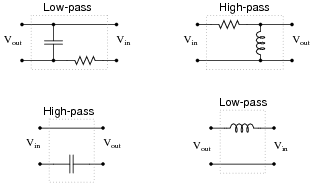
\includegraphics[width=\linewidth, height=50mm]{images/HiLoPass.png}
      \tiny \url{http://www.learningelectronics.net/images/quiz/00615x02.png}
            \end{minipage}

 \\ \hline
}

%%%%%%%%%%%%%%%%%%%%%%%%%%%%%%%%%%%%%%%

\subsection{Magnetic and electric fields in matter}
\Table{
\hline

Dipole moment & $ \bold{p} = \alpha\bold{E} $, where $\alpha$ is atomic polarizability.

\\ \hline

Polarization & $\bold{P} = \bold{p} \ / $ unit volume

\\ \hline

Bound charge 	& $ \sigma_b = \bold{P} \cdot \hat n,  \ \ \ \ \ \rho_b = - \pmb{\nabla} \cdot \bold{P}$

\\ \hline

Electric displacement field & $\bold{D} = \epsilon_0 \bold{E} + \bold{P} = \epsilon \bold{E}$

 \\ \hline
}

%%%%

\Table{
\hline

Gauss's Law in L.D.

&

\MiniPg{.6}{
\center

$\epsilon_0 \nabla \cdot \bold{E} = \rho = \rho_b + \rho_f = - \nabla \cdot \bold{P} + \rho_f$

$\nabla \cdot (\epsilon_0 \bold{E} + \bold{P}) = \nabla \cdot \bold{D} = \rho_f$

}

\\ \hline
}

%%%%

\Table{
\hline

Polarization in linear dielectrics 	& $\bold{P} = \epsilon_0 \chi_e \bold{E}$, where $\chi_e$ is the electric susceptibility.

\\ \hline

$ \bold{D} $ in terms of $\chi_e$ 	& $\bold{D} = \epsilon_0 (1 + \chi_e)\bold{E} = \epsilon \bold{E}$, where permittivity $\epsilon \equiv \epsilon_0 (1 + \chi_e) $

\\ \hline

Dielectric constant	& $\epsilon_r \equiv 1 + \chi_e \equiv \epsilon / \epsilon_0 $, (a.k.a. relative permittivity)

\\ \hline
}

%%%%

\Table{
\hline

$\bold{E} $ in dielectric  filled space & 
\MiniPg{.6}{\center
$\dfrac{1}{\epsilon_r} \bold{E}_{vac}$
}
\\ \hline

E-field in capacitor with dielectric

&

$E = \Delta V / d$

\\ \hline

Capacitance with linear dielectric

&

$C = \epsilon_r C_{\textrm{vac}}$

\\ \hline
}

%%%%

\Table{
\hline

Boundary conditions 	& $\epsilon_aE_a^\bot -\epsilon_bE_b^\bot = \sigma_f $ \\
				& $ V(a) = V(b) $
				
\\ \hline
}

%%%%%%%%%%%%%

\Table{
\hline

Magnetic dipole moment	& $\bold{m} = I \bold{a} $

\\ \hline

Magnetization	& $\bold{M} \equiv \bold{m} / $ unit volume

\\ \hline
}

%%%%

\Table{
\hline

$H$ field	& $\bold{H} \equiv \dfrac{1}{\mu_0} \bold{B} - \bold{M} $\\
		& $\pmb{\nabla} \times \bold{H} = \bold{J}_f $ \\
		& $\pmb{\nabla} \cdot \bold{H} = -\pmb{\nabla} \cdot \bold{M} $\\
		& Generally, $\bold{H} \parallel \bold{B} \parallel \bold{M} $.

\\ \hline
}

%%%%

\Table{
\hline

Linear magnetic materials	& $\bold{M} = \chi_m \bold{H} $ \\
					& where $\chi_m = $ magnetic susceptibility.

\\ \hline
}

%%%%

\Table{
\hline

B-field in linear	mag. material 	& $\bold{B} = \mu_0(1+\chi_m)\bold{H} = \mu \bold{H} $ \\
						& where $\mu \equiv \mu_0(1+\chi_m) = $ magnetic permeability. \\
						& $B_{material} = \dfrac{\mu}{\mu_0}B_{vacuum} = \mu_r B_{vacuum} $ \\
						& where $\mu_r \equiv \mu / \mu_0 = $ relative permeability.


\\ \hline
}

%%%%%%%%%%%%%

\Table{
\hline

Hall effect & 
\begin{minipage}{.55\textwidth}
      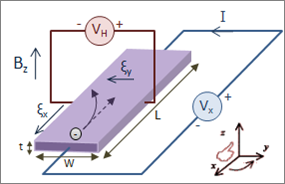
\includegraphics[width=\linewidth, height=50mm]{images/HallEffect.png}
            \end{minipage}
            \\
            &
            \tiny \url{https://en.wikipedia.org/wiki/Hall_effect}

\\ \hline
}

%%%%

\Table{
\hline

Hall voltage for electrons & $V_H = v_xB_zw $ and $I_x = ntw(-vx)(-e) $\\
& $V_H = \dfrac{I_x B_z}{nte}$

\\ \hline
}

%%%%

\Table{
\hline

Hall coefficient for electrons & $R_H = \dfrac{E_y}{j_x B} = \dfrac{V_H t}{I B} = - \dfrac{1}{ne}$ \\
& $[R_H] = $m$^3$/C

\\ \hline
}


